\documentclass[a4paper,twoside]{article}
\usepackage[T1]{fontenc}
\usepackage[bahasa]{babel}
\usepackage{graphicx}
\usepackage{graphics}
\usepackage{float}
\usepackage[cm]{fullpage}
\pagestyle{myheadings}
\usepackage{etoolbox}
\usepackage{setspace} 
\usepackage{lipsum}

% Custom packages
\usepackage[]{hyperref} % links
\usepackage{subcaption} % subfigure
\usepackage{verbatim} % block comment
\usepackage{xspace} % force space

\setlength{\headsep}{30pt}
\usepackage[inner=2cm,outer=2.5cm,top=2.5cm,bottom=2cm]{geometry} %margin
% \pagestyle{empty}

\makeatletter
\renewcommand{\@maketitle} {\begin{center} {\LARGE \textbf{ \textsc{\@title}} \par} \bigskip {\large \textbf{\textsc{\@author}} }\end{center} }
\renewcommand{\thispagestyle}[1]{}
\markright{\textbf{\textsc{Laporan Perkembangan Pengerjaan Skripsi\textemdash Sem. Genap 2021/2022}}}

\graphicspath{{./Gambar/}}% folder tempat gambar 
%untuk url dan link
\hypersetup{unicode=true,colorlinks=true,linkcolor=blue,citecolor=green,filecolor=magenta, urlcolor=cyan}

\onehalfspacing

\hyphenation{me-ngu-rangi}
\hyphenation{ma-sya-ra-kat}
\hyphenation{com-mand}
\hyphenation{line}
\hyphenation{me-nam-pil-kan}
\hyphenation{pe-rang-kat}
\hyphenation{kom-pu-ter}
 
\begin{document}

\title{\@judultopik}
\author{\nama \textendash \@npm} 

%ISILAH DATA BERIKUT INI:
\newcommand{\nama}{Alfred Aprianto Liaunardi}
\newcommand{\@npm}{6181801014}
\newcommand{\tanggal}{20/03/2022} %Tanggal pembuatan dokumen
\newcommand{\@judultopik}{Perkakas Command Line KIRI} % Judul/topik anda
\newcommand{\kodetopik}{PAN5201}
\newcommand{\jumpemb}{1} % Jumlah pembimbing, 1 atau 2
\newcommand{\pembA}{Pascal Alfadian Nugroho, M.Comp.}
\newcommand{\pembB}{-}
\newcommand{\semesterPertama}{52 - Genap 21/22} % semester pertama kali topik diambil, angka 1 dimulai dari sem Ganjil 96/97
\newcommand{\lamaSkripsi}{1} % Jumlah semester untuk mengerjakan skripsi s.d. dokumen ini dibuat
\newcommand{\kulPertama}{Skripsi 1} % Kuliah dimana topik ini diambil pertama kali
\newcommand{\tipePR}{B} % tipe progress report :
% A : dokumen pendukung untuk pengambilan ke-2 di Skripsi 1
% B : dokumen untuk reviewer pada presentasi dan review Skripsi 1
% C : dokumen pendukung untuk pengambilan ke-2 di Skripsi 2

% New words/phrases
\newcommand{\chromewebstorecli}{\textit{Chrome Web Store Item Property CLI}\xspace}
\newcommand{\cl}{\textit{command line}\xspace}
\newcommand{\cli}{\textit{command line interface}\xspace}
\newcommand{\itunesapi}{\textit{iTunes Search API}\xspace}
\newcommand{\latlon}{\textit{latitude} dan \textit{longitude}\xspace}

% Custom commands
\renewcommand{\refname}{Daftar Referensi}

% Dokumen hasil template ini harus dicetak bolak-balik !!!!

\maketitle

\pagenumbering{arabic}

\section{Data Skripsi} %TIDAK PERLU MENGUBAH BAGIAN INI !!!
Pembimbing utama/tunggal: {\bf \pembA}\\
Pembimbing pendamping: {\bf \pembB}\\
Kode Topik : {\bf \kodetopik}\\
Topik ini sudah dikerjakan selama : {\bf \lamaSkripsi} semester\\
Pengambilan pertama kali topik ini pada : Semester {\bf \semesterPertama} \\
Pengambilan pertama kali topik ini di kuliah : {\bf \kulPertama} \\
Tipe Laporan : {\bf \tipePR} -
\ifdefstring{\tipePR}{A}{
			Dokumen pendukung untuk {\BF pengambilan ke-2 di Skripsi 1} }
		{
		\ifdefstring{\tipePR}{B} {
				Dokumen untuk reviewer pada presentasi dan {\bf review Skripsi 1}}
			{	Dokumen pendukung untuk {\bf pengambilan ke-2 di Skripsi 2}}
		}
		
\section{Latar Belakang}
Project KIRI\footnote{\href{https://projectkiri.id}{https://projectkiri.id}} (akan disingkat sebagai KIRI dalam dokumen ini) adalah sebuah perangkat lunak berbasis web yang dibuat untuk \mbox{membantu} mengurangi efek dari kemacetan. KIRI mengurangi dampak kemacetan dengan membantu penggunanya, baik \mbox{masyarakat} maupun turis, dalam menggunakan salah satu sarana transportasi umum yang ada di Indonesia, yaitu angkutan kota (angkot). Cara KIRI \mbox{mempermudah} penggunaan angkot adalah dengan menunjukkan rute yang akan ditempuh, beserta langkah-langkah yang harus dilakukan oleh pengguna yang ingin berpergian dari satu titik ke titik lain, mulai dari seberapa jauh pengguna harus berjalan untuk menaiki angkot yang bersangkutan, di mana pengguna harus naik atau turun, seberapa jauh lagi pengguna harus berjalan sampai ke titik tujuan, dan seberapa lama estimasi waktu perjalanan yang akan ditempuh. Untuk kebutuhan pembuatan perangkat lunak yang memanfaatkan fitur dari KIRI, tersedia juga REST API KIRI yang dapat digunakan secara praktis. Adapun tampilan dari halaman web ini dapat dilihat di gambar \ref{fig:kiri-page}. 

\begin{figure}[ht]
    \centering
    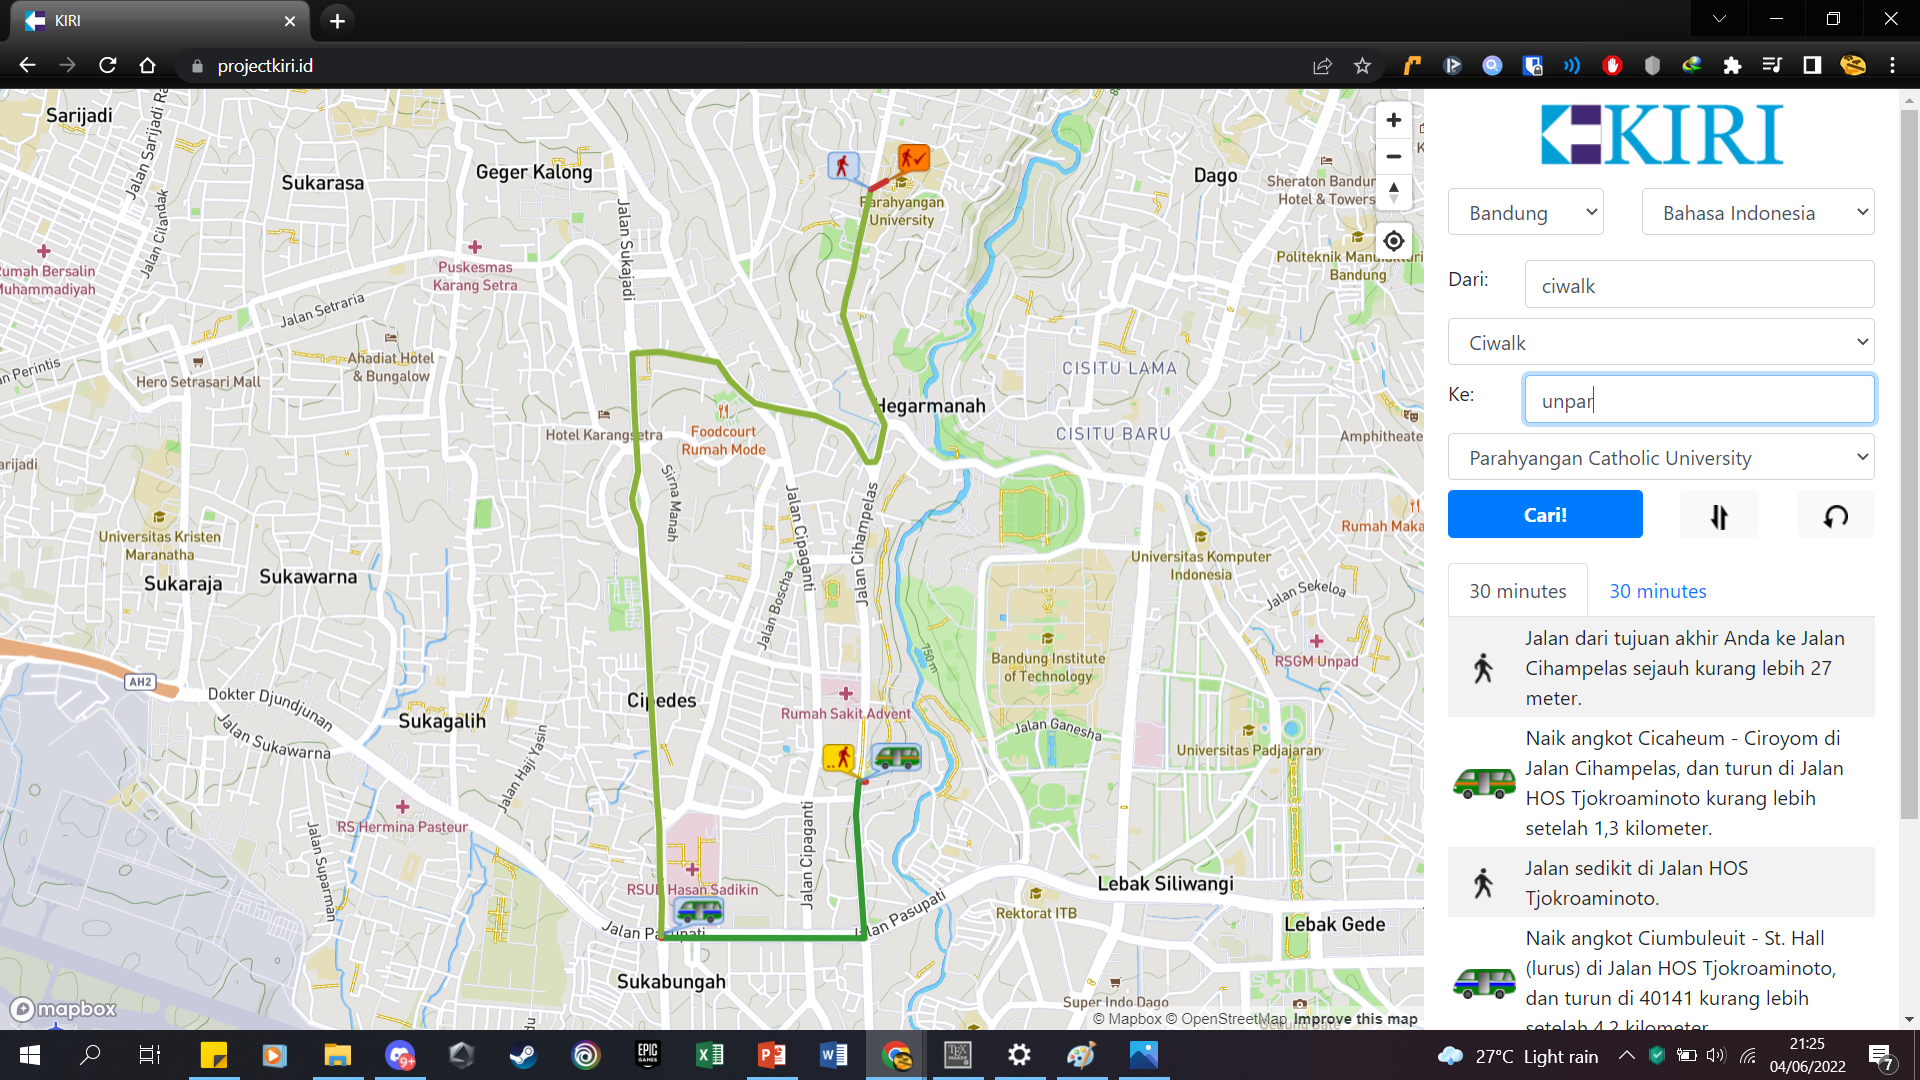
\includegraphics[width=0.74\linewidth]{projectkiri-example}
    \caption[Tampilan halaman web KIRI]{Tampilan halaman web KIRI, yang menunjukkan rute dari Cihampelas Walk ke Universitas Katolik Parahyangan.}
    \label{fig:kiri-page}
\end{figure}

Sementara itu, dalam komputer, salah satu dari sekian banyak tipe perangkat lunak adalah \textit{command line}. \textit{\mbox{Command} line} (\cl \textit{interpreter}, atau \cl \textit{interface}) adalah sebuah perangkat lunak berupa sebuah kotak/\textit{window} yang memuat teks berupa perintah-perintah,\footnote{\href{https://ubuntu.com/tutorials/command-line-for-beginners\#3-opening-a-terminal}{Ubuntu Tutorials - The Linux command line for beginners: 3. Opening a Terminal}} yang menerima masukan dari pengguna dan  menjalankannya.\cite{marsh:2010:fatfreeintrotocommandline} Perintah-perintah ini hanya berupa gabungan dari teks and simbol-simbol berupa karakter, tanpa ada tambahan gambar grafis apapun. Singkatnya, tipe perangkat lunak ini bukan merupakan tipe yang paling indah untuk dilihat oleh para pengguna, tetapi jika digunakan dengan tepat, maka \mbox{jenis} \mbox{perangkat} lunak ini bisa menyuruh komputer untuk melakukan banyak sekali perintah-perintah dengan sangat cepat dan sangat efektif.

Pada skripsi ini akan dibuat sebuah perangkat lunak berupa perkakas \cl (\textit{command line tool}) yang dapat menjalankan fungsi-fungsi API dari KIRI. Perangkat lunak ini, seperti jenisnya, akan dibuat murni sebagai perkakas yang dijalankan dari \cl (terminal, cmd, PowerShell, dll.), dan tampilan akhir dari perangkat lunak akan berupa \cli tanpa tambahan \textit{graphical user interface}. Keseluruhan dari perangkat lunak ini akan dibangun dalam bahasa C.

\section{Rumusan Masalah}
\begin{enumerate}
	\item Bagaimana membangun perkakas \textit{command line} yang dapat mengimplementasikan fitur-fitur API KIRI dalam bahasa C?
	\item Bagaimana integrasi perkakas \textit{command line} KIRI dapat dilakukan dengan perkakas-perkakas \textit{command line} lainnya di Linux?
\end{enumerate}

\section{Tujuan}
\begin{enumerate}
	\item Membangun perkakas \textit{command line} yang dapat mengimplementasikan fitur-fitur API KIRI dalam bahasa C.
	\item Melakukan integrasi perkakas \textit{command line} KIRI dengan perkakas-perkakas \textit{command line} lainnya di Linux.
\end{enumerate}

\section{Deskripsi Perangkat Lunak}
Perangkat lunak akhir yang akan dibuat memiliki fitur minimal sebagai berikut:
\begin{itemize}
	\item Pengguna dapat memasukkan lokasi awal dan tujuan akhir sebagai masukan dari perangkat lunak.
	\item Pengguna dapat melihat langkah-langkah yang harus ditempuh dalam perjalanan, mulai dari angkot mana saja yang harus dinaiki, ke mana pengguna harus berjalan kaki untuk bisa mencapai angkot terdekat dari lokasi terakhir pengguna, sampai seberapa jauh pengguna harus berjalan untuk mencapai tujuan akhir.
	\item Pengguna dapat melihat jarak yang harus ditempuh untuk setiap langkahnya.
	\item Pengguna dapat melihat seberapa lama waktu perjalanan untuk setiap langkahnya.
\end{itemize}


\section{Detail Perkembangan Pengerjaan Skripsi}
Detail bagian pekerjaan skripsi sesuai dengan rencan kerja/laporan perkembangan terkahir :
	\begin{enumerate}
		\item \textbf{Melakukan eksplorasi fungsi-fungsi perangkat lunak KIRI serta eksplorasi cara \mbox{implementasi} API KIRI.}\\
		{\bf Status :} Ada sejak rencana kerja skripsi.\\
		{\bf Hasil :} KIRI merupakan sebuah perangkat lunak berbasis web yang berfungsi untuk menyelesaikan (atau setidaknya mengurangi) dampak dari masalah-masalah yang dapat diselesaikan oleh \mbox{transportasi} umum/publik di Indonesia, seperti pemanasan global, kemacetan, atau peningkatan harga bensin. Selain itu, turis mancanegara juga memilih untuk menaiki transportasi umum, karena jenis sarana transportasi tersebut tidak hanya jauh lebih murah, tetapi juga memberikan kesempatan yang mudah kepada mereka untuk melihat seluk-beluk dari kota-kota yang mereka kunjungi.\footnote{\href{https://projectkiri.github.io/\#about-kiri}{https://projectkiri.github.io/\#about-kiri}}

Di halaman web KIRI, pengguna dapat memasukkan input berupa lokasi awal dan lokasi tujuan dan KIRI akan menghasilkan seluruh langkah yang harus ditempuh oleh pengguna untuk sampai ke lokasi tujuan, dengan menggunakan angkot. Keluaran ini sudah meliputi kode angkot mana saja yang harus dinaiki, dan juga seberapa jauh pengguna harus berjalan kaki untuk sampai ke lokasi rute angkot berikutnya.

KIRI juga memiliki sebuah API yang dapat digunakan untuk keperluan pengembangan perangkat lunak. Seluruh permintaan (\textit{request}) yang dilakukan melalui API KIRI harus dilakukan sebagai \mbox{permintaan} tipe GET ke \href{https://projectkiri.id/api}{https://projectkiri.id/api}, beserta parameter-parameter yang dibutuhkan. 
\newline\newline
Permintaan tersebut harus memiliki parameter-parameter seperti terlihat di bawah ini.\footnote{\href{https://github.com/projectkiri/Tirtayasa/wiki/KIRI-API-v2}{https://github.com/projectkiri/Tirtayasa/wiki/KIRI-API-v2}}

\begin{itemize}
	\item \verb|version|\\
	\textbf{Kemungkinan nilai:} \verb|2|\\
	Parameter ini merupakan tanda bagi API untuk menggunakan protokol versi 2.
	\item \verb|mode|\\
	\textbf{Kemungkinan nilai:} \verb|findroute|\\
	Parameter ini merupakan mode dari servis/jasa API yang akan digunakan oleh pengguna. Untuk mode \verb|findroute|, jasa yang akan digunakan adalah jasa pencarian rute dengan angkot.
	\item \verb|locale|\\
	\textbf{Kemungkinan nilai:} \verb|en| atau \verb|id|\\
	Parameter ini mengatur bahasa apa yang akan digunakan dalam keluaran API nantinya\textemdash\verb|en| berarti keluaran akan menggunakan bahasa Inggris, dan \verb|id| berarti keluaran akan menggunakan bahasa Indonesia.
	\item \verb|start|\\
	\textbf{Kemungkinan nilai:} \verb|lat|, \verb|lng|; dalam bentuk desimal\\
	Parameter ini merupakan nilai \latlon dari titik awal perjalanan pengguna.
	\item \verb|finish|\\
	\textbf{Kemungkinan nilai:} \verb|lat|, \verb|lng|; dalam bentuk desimal\\
	Parameter ini merupakan nilai \latlon dari titik akhir/tujuan perjalanan pengguna.
	\item \verb|presentation|\\
	\textbf{Kemungkinan nilai:} \verb|desktop|\\
	Parameter ini hanya digunakan untuk fitur \textit{backwards compatibility}.
	\item \verb|apikey|\\
	\textbf{Kemungkinan nilai:} angka heksadesimal 16-digit\\
	Parameter ini berisi kunci API pribadi yang harus digenerasi terlebih dahulu sebelum API dapat digunakan.
\end{itemize}
% \vspace{\baselineskip}
Sedangkan, respon yang diberikan oleh API berupa sebuah objek JSON yang selalu memiliki setidaknya dua variabel, yaitu:\footnote{\href{https://github.com/projectkiri/Tirtayasa/wiki/KIRI-API-v2}{https://github.com/projectkiri/Tirtayasa/wiki/KIRI-API-v2}}

\begin{itemize}
	\item \verb|status|\\
	\textbf{Kemungkinan nilai:} \verb|ok| atau \verb|error|\\
	Variabel ini manandakan apakah permintaan berhasil diproses atau tidak. Jika permintaan berhasil diproses, variabel ini akan bernilai \verb|ok|, dan jika tidak, variabel ini akan bernilai \verb|error|.
	\item \verb|message|\\
	Variabel ini bisa berisi dua macam objek. Jika permintaan dari user tidak berhasil diproses, atau dalam kata lain, terjadi sebuah \textit{error}, maka variabel ini akan berisi string yang merupakan pesan \textit{error} serta alasan spesifik mengapa \textit{error} tersebut terjadi. Di lain sisi, jika permintaan dari user berhasil diproses, variabel ini akan mengalami dua perubahan utama. Pertama, nama variabel ini akan berubah menjadi \verb|routingresults|, dan kedua, isi dari variabel ini akan menjadi sebuah \textit{array} JSON yang merupakan respon dari API KIRI berupa keluaran yang akan dilihat oleh pengguna. \textit{Array} JSON ini sendiri terbagi menjadi beberapa variabel lainnya, yang dapat dilihat di daftar di bawah ini.
	
	\begin{itemize}
		\item \verb|steps|\\
		\textbf{Tipe:} array\\
		Variabel ini merepresentasikan satu buah langkah yang harus ditempuh oleh pengguna. Adapun \textit{array} ini sendiri berisi variabel-variabel berikut:
		
		\begin{itemize}
			\item Tipe transportasi\\
			Tipe sarana transportasi yang harus dipakai oleh pengguna. Jika pengguna harus berjalan kaki, variabel ini akan berisi \verb|walk|. Jika pengguna harus menaiki angkot, variabel ini akan berisi \verb|angkot|.
			\item Kode angkot\\
			Variabel ini menunjukkan angkot mana yang harus dinaiki oleh pengguna di langkah tersebut. Jika penggunaan angkot tidak dimungkinkan pada langkah ini (pengguna harus berjalan kaki), variabel ini akan berisi \verb|walk|.
			\item Array \latlon lokasi\\
			\textit{Array} nilai-nilai desimal \latlon dari berbagai titik lokasi yang terdapat dalam rute.
			\item Deskripsi langkah\\
			Deskripsi langkah yang harus ditempuh, dalam bahasa natural. Bahasa yang digunakan tergantung parameter \verb|locale| yang diatur dalam masukan.
			\item URL untuk mendapatkan tiket kendaraan\\
			Tautan untuk mendapatkan tiket angkutan umum, jika diperlukan. Jika transportasi pada langkah tersebut tidak memerlukan tiket, variabel ini akan berisi \verb|null|.
			\item URL editor rute\\
			Tautan untuk meng-edit rute, jika situasinya memungkinkan. Jika tidak, variabel ini akan berisi \verb|null|.
		\end{itemize}
		
		\item \verb|traveltime|\\
		\textbf{Tipe:} string\\
		Variabel ini berisi estimasi jangka waktu yang diperlukan untuk menyelesaikan langkah tersebut.
	\end{itemize}
	
\end{itemize}
		
		\item \textbf{Mempelajari perkakas-perkakas \cl sejenis.}\\
		{\bf Status :} Ditambahkan pada Skripsi 1.\\
		{\bf Hasil :} Perkakas-perkakas sejenis yang dianalisis meliputi \chromewebstorecli dan \textit{iTunes Search API}.

\begin{itemize}
	\item \chromewebstorecli\\
	Perkakas ini dapat digunakan melalui \textit{command prompt} dengan cara mengetikkan perintah sebagai berikut.

	\begin{verbatim}
                     chrome-web-store-item-property <identifier>
	\end{verbatim}

	Dengan \verb|identifier| berupa ID dari ekstensi yang diinginkan. Jadi, misalkan pengguna memasukkan \verb|gighmmpiobklfepjocnamgkkbiglidom| sebagai ID yang akan digunakan sebagai \textit{identifier}, maka perkakas ini akan mengembalikan metadata dari ekstensi ``AdBlock'' sebagai keluarannya. Contoh penggunaan perkakas ini dapat dilihat di gambar \ref{fig:similarapps-chromewebstorecli}.

	\begin{figure}[ht]
	    \centering
	    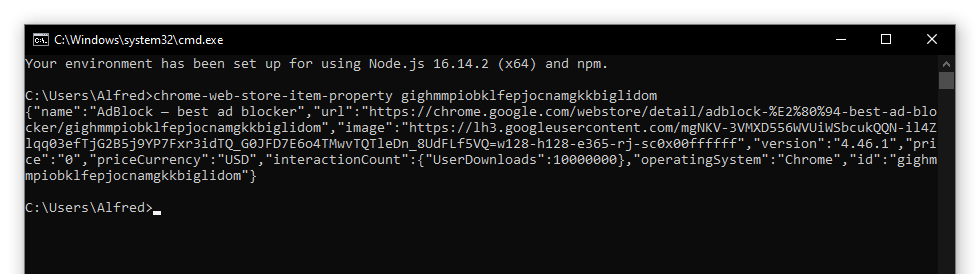
\includegraphics[width=0.75\linewidth]{chromewebstorecli}
	    \caption[Contoh penggunaan perkakas \chromewebstorecli]{Contoh penggunaan perkakas \chromewebstorecli.}
    	\label{fig:similarapps-chromewebstorecli}
	\end{figure}
	
	Sedangkan, keluaran dari perkakas ini merupakan sebuah objek JSON dengan properti-properti sebagai berikut.
	
	\begin{itemize}
		\item \verb|name|\\
		Nama dari ekstensi yang dicari metadatanya.
		\item \verb|url|\\
		URL halaman web dari ekstensi yang dicari di \textit{web store} Google Chrome.
		\item \verb|image|\\
		Logo (dan ikon \textit{thumbnail}) dari ekstensi yang dicari metadatanya.
		\item \verb|version|\\
		Nomor versi dari ekstensi.
		\item \verb|price|\\
		Harga dari ekstensi. Jika ekstensi tidak memiliki harga yang perlu dibayarkan (gratis), properti ini akan bernilai \verb|0|.
		\item \verb|priceCurrency|\\
		Kode mata uang dari harga ekstensi. Jika ekstensi tidak memiliki harga yang perlu dibayarkan, properti ini akan berisi ``\verb|USD|``.
		\item \verb|interactionCount|\\
		Properti ini berisi interaksi-interaksi pengguna yang tercatat sebagai data di halaman \textit{web store} ekstensi. Pada saat pembuatan skripsi ini, properti ini hanya memiliki satu buah subproperti, yaitu \verb|userDownloads|, yang menandakan berapa kali ekstensi ini telah diunduh oleh pengguna di manapun.
		\item \verb|operatingSystems|\\
		Menandakan di peramban mana ekstensi versi ini dapat diinstal. Karena ekstensi-ekstensinya berada di \textit{web store} Chrome,
		\item \verb|ratingValue| (tidak digunakan lagi)\\
		Peringkat yang diberikan oleh para pengguna ekstensi ini. Nilai dari properti ini berupa skala desimal dari 0.00 sampai dengan 5.00. Di versi terbaru dari perkakas ini, properti ini tidak lagi tersedia dalam keluarannya.
	\item \verb|ratingCount| (tidak digunakan lagi)\\
		Jumlah pengguna yang telah menilai/memberi peringkat ke ekstensi ini. Di versi terbaru dari perkakas ini, properti ini tidak lagi tersedia dalam keluarannya.
		\item \verb|id|\\
		Properti ini mengandung ID dari ekstensi tersebut. Nilai dari properti ini akan sama dengan ID yang digunakan sebagai parameter masukan perkakas.
	\end{itemize}
	
	\item \itunesapi\\
	Perkakas \cl ini berfungsi untuk melakukan pencarian melalui API iTunes, sehingga seakan-akan pengguna langsung melakukan pencarian di iTunes sendiri. Hasil pencarian yang dilakukan termasuk judul lagu, nama artis, ataupun nama album, dan pengguna dapat memilih secara spesifik objek apa yang ingin dicari.

	Perkakas ini dapat digunakan melalui \textit{command prompt} dengan cara mengetikkan perintah sebagai berikut.
	
	\begin{verbatim}
                      itunes-search-api <input> [<options>]
	\end{verbatim}
	
	Dengan \verb|input| berupa nama dari objek yang dicari. Perkakas ini juga memiliki opsi yang masing-masing memiliki parameter tersendiri untuk mempersempit hasil pencarian. Adapun opsi-opsi tersebut dapat dilihat di daftar di bawah ini.
	
	\begin{itemize}
		\item \verb|country|\\
		\textbf{Kemungkinan nilai:} Kode negara dua huruf\\
		Opsi ini menerima parameter berupa kode negara asal dari album atau artis yang dicari.
		\item \verb|entity|\\
		\textbf{Kemungkinan nilai:} \verb|song|, \verb|musicArtist|, atau \verb|album|\\
		Menandakan jenis objek/entitas yang ingin dicari. Opsi ini dapat bernilai \verb|song| untuk pencarian berbasis judul lagu, \verb|musicArtist| untuk pencarian nama artis, atau \verb|album| untuk pencarian nama album. Jika opsi ini tidak dipakai, objek apapun yang memiliki kemiripan dengan \verb|input| dalam salah satu dari ketiga properti ini akan muncul dalam hasil pencarian.
		\item \verb|limit|\\
		\textbf{Kemungkinan nilai:} Bilangan bulat positif\footnote{Opsi ini juga menerima bilangan bulat negatif, tetapi menggunakan sebuah bilangan bulat negatif akan menghilangkan pengaruh opsi ini terhadap hasil keluaran.}\\
		Jumlah hasil pencarian maksimal yang ingin ditampilkan dalam keluaran.
	\end{itemize}
	\vspace{\baselineskip}
	Sedangkan, keluaran dari perkakas ini merupakan sebuah objek JSON yang memiliki dua properti utama, yaitu:
	
	\begin{itemize}
		\item \verb|resultCount|\\
		Properti ini berisi bilangan bulat yang menandakan berapa buah objek yang terdapat dalam hasil pencarian.
		\item \verb|results|\\
		\textit{Array} yang berisi kumpulan objek yang terdapat di dalam hasil pencarian. Objek-objek ini akan dikembalikan berupa sebuah \textit{array} lain yang berisi seluruh properti dari masing-masing objek. Apa saja properti yang diikutkan dalam \textit{array} tersebut tergantung tipe dari objek dalam hasil pencarian.
	\end{itemize}
	
	\begin{figure}[ht]
	    \centering
	    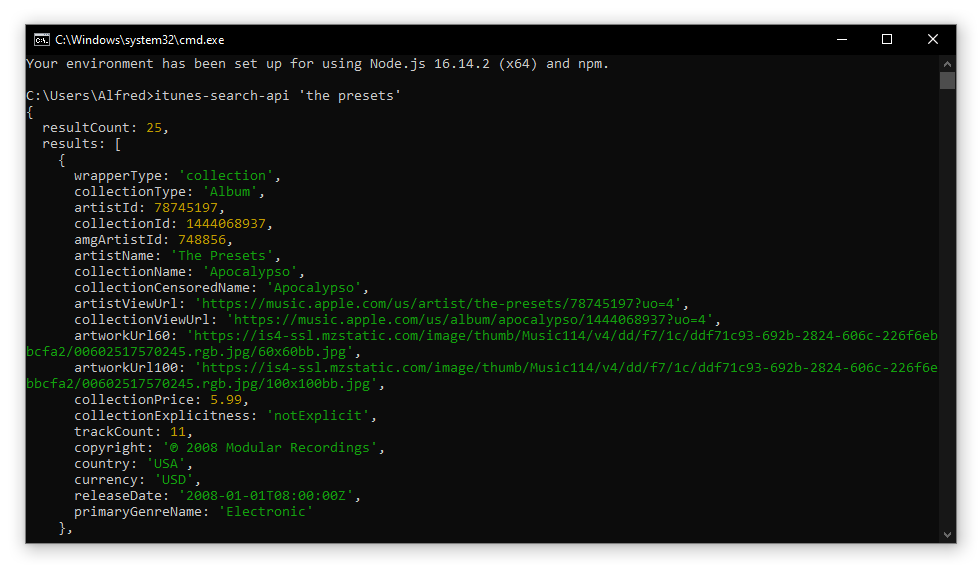
\includegraphics[width=0.75\linewidth]{itunesapi}
	    \caption[Contoh penggunaan perkakas \itunesapi]{Contoh penggunaan perkakas \itunesapi. Gambar hanya memuat satu objek untuk menghemat tempat.}
    	\label{fig:itunesapi}
	\end{figure}
	\vspace{\baselineskip}
	Adapun contoh penggunaan dan hasil keluaran perkakas ini dapat dilihat di gambar \ref{fig:itunesapi}.


\end{itemize}
		
		\item \textbf{Mempelajari bahasa pemrograman C serta mempelajari dokumentasi-dokumentasi dari seluruh modul yang dibutuhkan untuk pembuatan perangkat lunak.}\\
		{\bf Status :} Ada sejak rencana kerja skripsi.\\
		{\bf Hasil :} Ada beberapa modul/fungsi bawaan dari bahasa C yang akan digunakan dalam pembuatan perkakas \cl ini. Salah satu dari fungsi tersebut adalah fungsi \verb|getopt|

		\item \textbf{Melakukan analisis dan desain perangkat lunak yang akan dibangun.}\\
		{\bf Status :} Ada sejak rencana kerja skripsi.\\
		{\bf Hasil :}

		\item \textbf{Melakukan analisis kebutuhan fitur-fitur perangkat lunak dan melakukan eksplorasi \textit{library} yang dapat digunakan dan memenuhi spesifikasi dalam pembuatan perangkat lunak.}\\
		{\bf Status :} Ada sejak rencana kerja skripsi.\\
		{\bf Hasil :}

		\item \textbf{Membangun perangkat lunak berdasarkan rancangan yang sudah dibuat, dengan megimplementasikan seluruh modul dan \textit{library} yang telah ditentukan di tahap sebelumnya dalam bahasa C.}\\
		{\bf Status :} Ada sejak rencana kerja skripsi.\\
		{\bf Hasil :} Poin ini akan dikerjakan di Skripsi 2.

		\item \textbf{Melakukan pengujian fungsional dan perbaikan \textit{bug}.}\\
		{\bf Status :} Ada sejak rencana kerja skripsi.\\
		{\bf Hasil :} Poin ini akan dikerjakan di Skripsi 2.
		
% Example of dropped step
%		\item \textbf{Melakukan pengujian fungsional dan perbaikan \textit{bug}.}\\
%		{\bf Status :} Tidak dikerjakan \\
%		{\bf Hasil :} Berdasarkan analisis singkat, tidak dilakukan analisis lebih jauh karena tidak diperlukan struktur data baru, karena sudah disediakan oleh OpenSteer versi terbaru

		\item \textbf{Menulis dokumentasi perangkat lunak.}\\
		{\bf Status :} Ada sejak rencana kerja skripsi.\\
		{\bf Hasil :} Poin ini akan dikerjakan di Skripsi 2.

		\item \textbf{Menulis dokumen skripsi.}\\
		{\bf Status :} Ada sejak rencana kerja skripsi.\\
		{\bf Hasil :} Dokumen skripsi akan ditulis hingga bab 3 pada Skripsi 1. Pengisian sisa dari dokumen skripsi, serta penyempurnaan bab 1 sampai bab 3, akan dilakukan pada Skripsi 2.

	\end{enumerate}

\section{Pencapaian Rencana Kerja}
Langkah-langkah kerja yang berhasil diselesaikan dalam Skripsi 1 ini adalah sebagai berikut:
\begin{enumerate}
\item
\item
\item
\end{enumerate}

%TULISKAN BAGIAN INI JIKA DOKUMEN ANDA TIPE A ATAU C
\begin{comment}
	\section{Kendala yang Dihadapi}
	Kendala - kendala yang dihadapi selama mengerjakan skripsi :
	\begin{itemize}
		\item Note: MASIH CONTOH!
		\item Terlalu banyak melakukan prokratinasi.
		\item Terlalu banyak godaan berupa hiburan (game, film, dll)
		\item Skripsi diambil bersamaan dengan kuliah ASD karena selama 5 semester pertama kuliah tersebut sangat dihindari dan tidak diambil, dan selama 4 semester terakhir kuliah tersebut selalu mendapat nilai E
		\item Mengalami kesulitan pada saat sudah mulai membuat program komputer karena selama ini selalu dibantu teman
	\end{itemize}
\end{comment}

\bibliographystyle{compj}
\bibliography{referensi} 

\vspace{1cm}
\centering Bandung, \tanggal\\
\vspace{2cm} \nama \\ 
\vspace{1cm}

Menyetujui, \\
\ifdefstring{\jumpemb}{2}{
\vspace{1.5cm}
\begin{centering} Menyetujui,\\ \end{centering} \vspace{0.75cm}
\begin{minipage}[b]{0.45\linewidth}
% \centering Bandung, \makebox[0.5cm]{\hrulefill}/\makebox[0.5cm]{\hrulefill}/2013 \\
\vspace{2cm} Nama: \pembA \\ Pembimbing Utama
\end{minipage} \hspace{0.5cm}
\begin{minipage}[b]{0.45\linewidth}
% \centering Bandung, \makebox[0.5cm]{\hrulefill}/\makebox[0.5cm]{\hrulefill}/2013\\
\vspace{2cm} Nama: \pembB \\ Pembimbing Pendamping
\end{minipage}
\vspace{0.5cm}
}{
% \centering Bandung, \makebox[0.5cm]{\hrulefill}/\makebox[0.5cm]{\hrulefill}/2013\\
\vspace{2cm} Nama: \pembA \\ Pembimbing Tunggal
}
\end{document}

